% Требование на модель
Разрешение циклических зависимостей графовой математической модели трассируемости требований к ПО на файлы исходного кода происходит в несколько этапов:
\begin{enumerate}
    \item считывание исходных данных;
    \item построение первичного графа трассируемости требований к ПО на файлы исходного кода приложения;
    \item пока в графе на слое файлов исходного кода присутствуют циклы выполнятся слияние входящих в цикл вершин;
    \item формирование результирующего графа трассируемости.
\end{enumerate}

Слияние входящих в цикл вершин следует производить итерационно до тех пор, пока в результирующем графе не будут отсутствовать циклы. После объединения вершин в одну группу граф видоизменяется. При этом для дуг, вершины которых объединяются, выполняется:
\begin{itemize}
    \item дуги между сливающимися вершинами удаляются;
    \item образованная группа является новой вершиной графа, при этом все входящие и исходящие дуги замыкаются на нее. Пример слияния приведен на рисунке~\ref{fig:merge_example};
\end{itemize}

\begin{figure}[H]
    \centering
    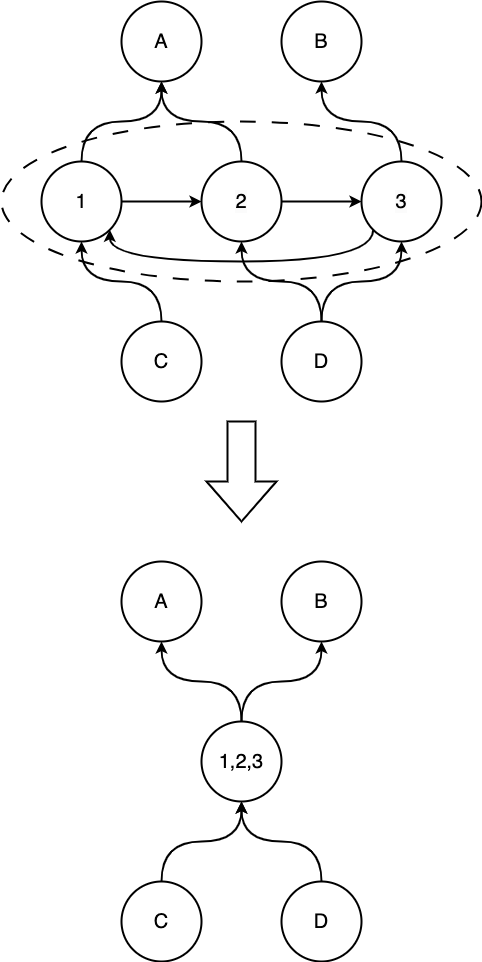
\includegraphics[width=0.5\textwidth]{merge_example}
    \caption{Пример слияния входящих в цикл вершин}
    \label{fig:merge_example}
\end{figure}

На следующей итерации поиска циклов в графе вышеобозначенные группы учитываются как обычные вершины и таким образом могут участвовать в образовании новых групп по вышеуказанным правилам.

Перед началом работы модели необходимо подготовить данные: все требования к ПО и файлы исходного кода программы должны быть проидентифицированы натуральными числами по возрастанию начиная с 1. В приводимых примерах литерой m обозначается максимальный идентификатор требования к ПО, литерой n обозначается максимальный идентификатор файла исходного кода.

Исходными данными для модели являются две матрицы бинарных отношений:
\begin{enumerate}
    \item матрица трассируемости требований на файлы исходного кода. В ней индекс столбца матрицы соответствует идентификатору требования, индекс строки - идентификатору файла исходного кода. Если файл исходного кода реализует требование, значение соответствующей элемента матрицы устанавливается равным 1, иначе 0 (рисунок~\ref{fig:requirements_traceability_matrix});
    \item матрица зависимостей между файлами исходного кода. В ней индексы столбцов и строк соответствуют идентификаторам файлов исходного кода. Значение элемента матрицы устанавливается равным 1 если файл исходного кода с идентификатором номера строки имеет зависимость на файл исходного кода с идентификатором номера столбца, иначе значение элемента устанавливается равным 0. В рамках решаемой задачи необходимость отображать зависимости файла исходного кода на самого себя отсутствует. В следствие этого, элементы матрицы на главной диагонали должны быть равны 0 (рисунок~\ref{fig:dependency_matrix}).
\end{enumerate}

\begin{figure}[H]
    \centering
    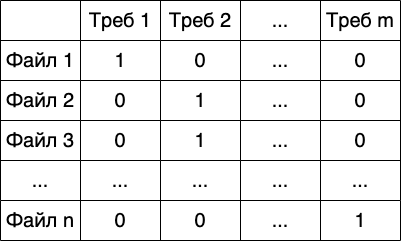
\includegraphics[width=0.5\textwidth]{requirements_traceability_matrix}
    \caption{Пример матрицы трассируемости требований на файлы исходного кода}
    \label{fig:requirements_traceability_matrix}
\end{figure}

\begin{figure}[H]
    \centering
    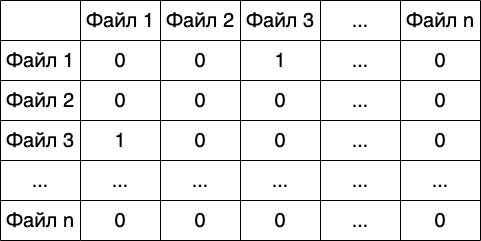
\includegraphics[width=0.6\textwidth]{dependency_matrix}
    \caption{Пример матрицы зависимостей файлов исходного кода друг на друга}
    \label{fig:dependency_matrix}
\end{figure}

По входным данным строится изначальный граф. В изначальном графе выделяются два слоя:
\begin{enumerate}
    \item слой файлов исходного кода
    \item слой требований к ПО
\end{enumerate}

Пример изначального графа, построенного по входным данным приведен на рисунке~\ref{fig:original_count}.

\begin{figure}[H]
    \centering
    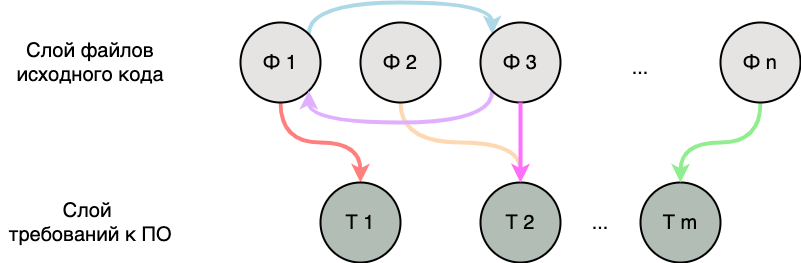
\includegraphics[width=1\textwidth]{original_count}
    \caption{Пример изначального графа}
    \label{fig:original_count}
\end{figure}

В приведенном примере вершины 1 и 3 образуют цикл. Результат слияния приведен на рисунке \ref{fig:result_count}.

\begin{figure}[H]
    \centering
    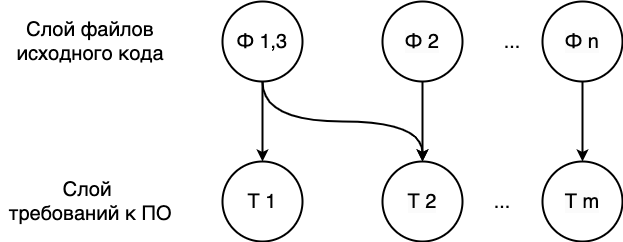
\includegraphics[width=0.8\textwidth]{result_count}
    \caption{Пример результирующего графа}
    \label{fig:result_count}
\end{figure}

Результирующий граф может быть использован при оценке объема верификационных процедур, которые необходимо выполнить при внесении изменений в файлы исходного кода. Так, при внесении изменений в файл исходного кода с идентификатором 1 требуется выполнить верификационные процедуры реализации требований с идентификаторами 1 и 2. Для этого необходимо выполнить тестовые процедуры относящиеся к файлам исходного кода с идентификаторами 1, 2 и 3.